% !TEX root = ../main.tex
%______________________________________________________________%
\section{Introduction}

\label{sec:intro}

% @J : intro needs lots of love.

The concept of the \emph{front-running} is decades old starting with early financial markets. Initially the traders required to be physically available in the exchange office to deliver the bids and offers, and some traders, in the knowledge of future market change, could run in front of the others to get their orders ahead of the change in the market to profit from the price change. Clearly in such scenarios front-running was possible yet not detectable as a damaging activity. However, with the rapid advances of the technology in the last few decades, trading is not carried out in person anymore, new form of front-running is feasible through high speed networks. Furthermore, Blockchain technology has introduced transparency and open markets and leads to a new era of front-running which inherently affects all decentral applications, whether financial or non-financial. Arbitrage and Censorship, are also issues that have been linked to front-running attacks on blockchain \textit{(We need to talk about why these two are left out of the scope of this paper)}. Currently, there are quite a few decentral applications built on the blockchains, so in order for us to perform a thorough study on blockchain application front-running, we set a s specific criteria by using the top 25 decentral applications which have the highest recent user activities.\footnote{List of decentralized applications \url{https://dappradar.com/dapps}} Using this criteria, we successfully categorized these decentral applications into 4 principal categories on which we conduct our analysis. Surprisingly, there was no ICO (initial coin offering) included in the top 25 Dapps list by the time we fetched the data from the website. We believe the reason is because the ICOs are inherently different from other groups of Daaps as they are merely highly active during their offering periods and their user activity drops dramatically after the offerings period are over. Therefore, we  consider ICOs as another cases on which the front-running should be investigated (although they are not listed in the top 25 Dapps we use) \footnote{A note to the reviewer: this paper falls under "Case Studies (\eg of adoption, attacks, forks, scams \etc)" and also mentions methods for "Fraud Detection and Financial Crime Prevention".}


%Decentral applications are on the rise with Turing complete blockchains maturing to handle high monetary value transactions. Tokenization mushroomed to a whole ecosystem of tokenized applications on the blockchain, these applications inherently become a market as tokens are in the core of them. We started looking at some of these applications, in specific \textit{Bancor}~\cite{hertzog2017bancor}, to look into possible issues rising from these new models. Transparency of blockchains, although being a good feature of them, opens up these markets to some attack vectors that might not be visible on the time of the application design, one main attack is known as \textbf{front-running}, whether financial or non-financial. Arbitrage and Censorship, are also issues arises from the designs on the blockchain technology and had been linked to front-running attacks, hence we use the term \textit{front-running] losely to talk about any transaction manupulation with the intention of getting other transactions in before the original transaction takes place. In this paper, our focus is to have a complete overview of front-running on the blockchain while analysing Bancor issues. While looking at the possibility of front-running on other applications, we found interesting case studies that affects most of the top 25 decentral applications on Ethereum blockchain.


%______________________________________________________________%
\section{Preliminaries}

\subsection{Traditional Front-running} 
\label{sec:What is front-running?}

\emph{Front-running} is analogous to any course of action during which a person or entity benefits from prior access to inside or confidential market information about upcoming transactions and trades, albeit the problem can occur in both financial and non-financial systems.  In traditional exchanges, traders would gather in same phsycal locations to announce their position in the market, in case of receiving a large order from a client, the broker might say this loud and other people around the table could be informed. Therefore, a malicious trader would run in front of that order and put his own transaction in-between (before the trade was executed) and hence profit from the price increase of the stock. 
%In fact, a group of market participants obtain non-public market information which allows them to front-run other user\'s trades by putting their orders ahead of those trades and benefit from advance knowledge of pending client orders. 
The two significant factors which cause the front-running practice to happen within the financial markets are (i) imperfect competition and (ii) liquidity uncertainty~\cite{liang2005distressed}. Any sort of front-running activity within the financial markets is considered as an unethical and illegal practice as it is unfairly beneficial for a few market participants who have the privilege of acting on this information and taking advantages at the expense of the investors. 

\subsection{Literature on Traditional Front-running}\label{traditionalFrontrunning}
As traditional front-running has been the subject of discussion for decades, there are many literatures on this subject. Here we focus on the historical context and how the regulations evolved to be what they are today.\\
Front-running was first appeared on the Chicago Board Options Exchange (\textit{CBoE})~\cite{markham1988front}, and was defined by \textit{Securities Exchange Commission} in 1977 as the following:
\begin{quote}
The practice of effecting an options transaction based upon non-public information regarding an impending block transaction\footnote{Block in the stock market is large number of shares, 10\,000 or more, to sell which will heavily changes the price} in the underlying stock, in order to obtain a profit when the options market adjusts to the price at which the block trades. ~\cite{sec1978optionsmarket}
\end{quote} 

% More to read:  SECURITIES AND EXCHANGE COMMISSION Release No. 34-67079. pdf included in Related_Documents
% https://www.sec.gov/about/annual_report/1988.pdf

On the years after there were ongoing discussions between self-regulatory exchanges (\eg \textit{CBoE}) and \textit{SEC} to regulate, detect and define laws and policies to deal with front-running~\cite{markham1988front}, with \textit{SEC} stating: 
\begin{quote}
It seems evident that such behaviour on the part of persons with knowledge of imminent transactions which will likely affect the price of the derivative security constitutes an unfair use of such knowledge. \footnote{Securities Exchange Act Release No. 14156, November 19, 1977, (Letter from George A. Fitzsimmons, Secretary, Securities and Exchange Commission to Joseph W. Sullivan, President  CBoE).}
\end{quote} 

Defining what exactly was considered illegal front-running required more knowledge of how these new markets behaved. \textit{CBoE} and other exchanges (and brokers) issued educational circulars for their members asserting that front-running violates existing rules, with some examples of what is considered front-running. However difference of opinion regarding the unfairness of front-running activities, insufficient exchange rules and lack of a precise definition in this area resulted in no action by self-regulator organizations~cite{sec1978optionsmarket}. 

Further reading on the early details on the history and challenges of detecting and regulating front-running is extensively written by Markham~\cite{markham1988front} . %add a more recent publication?

Initially the front-running policies only applied to certain option markets, later on in 2002, the rule was refined to include the same prohibitions to security futures~\cite{finra_2002},  then again in 2012 with the new amendment, FINRA Rule 5270, the front-running rule was extended to cover trading in options, derivatives, or other financial instruments overlying a security with a few exceptions~\cite{sec2012frontrunning, finra_2012}.


\subsection{Blockchain Front-running} \label{sec:Front Running on the Blockchains}

% everything that has a line up , someone can jump in the line and front-run

Blockchain technology has received an exceptional amount of attention since it was first introduced as the underlying technology of the cryptocurrency Bitcoin in 2008~\cite{nakamoto2008bitcoin}. Many decentralized applications that are built on top of this technology represent the significance of the blockchain as it completely eliminates the central point of failure within the systems. However, blockchains have some inherent characteristic that leave them vulnerable to information leaks and \emph{front-running} behaviour. Although this data structure is known to be publicly visible to every network participants, information is layered and some of them are easier accessed only by insiders. Any network participants that runs a full node on the blockchain is able to obtain those information and as mentioned in section~\ref{sec:What is front-running?}, this leaves the application vulnerable to front-running. %Decentralized exchanges are a group of blockchain financial applications where front-running can be executed. 
%____________________________________________________________________
%%% The following chunk seem to be redundant and weird. Should we keep it?? 
Bancor \cite{hertzog2017bancor} is an example of such systems in which front-runners benefit from potential price increase of the market stocks (details are provided in~\ref{sec:frontrunningExchanges}). Decentralized namespaces, as blockchain non-financial applications, are another example. Ethereum Name Service and Ghazal \cite{moosavighazal} are such systems in which upon seeing a transaction from Alice to register \texttt{alice.eth}, front-runner can go ahead of her and register this domain name. He can later sell \texttt{alice.eth} to Alice for a higher price and profit.
Another application that is vulnerable to front-running is Initial Coin Offering (ICO) smart contracts. ICO is a method to distribute tokens based on the deposits of the native coin, Ether in the case of Ethereum. After a few hacking incidents of high valued smart contracts~\cite{siegel2016daohack}, ICOs started to implement restrictions and capped how much funds can be gathered. This scarcity of the initial coins made for a competition to incentivize big investors to get in and buy the tokens at a discounted price and sell them to late comers on the open markets~\cite{zetzsche2018ico, li2018initial}. ICOs started to experiment with different fair capping methods, such as reverse dutch auction and dynamic ceilings~\cite{kaal2017initial}.  This competition made ICOs a good opportunity for front-running attacks.  In this paper we use multiple empirical examples to show possibility of front-running on DApps. For the sake of completeness, we use one incident on ICOs, and examples from the Top 25 DApps by recent user counts based on \texttt{DAppRadar.com} ranking. 
%____________________________________________________________________

\subsection{Literature on Blockchain Front-running}

Due to the novelty characteristics of the underlying technology (blockchain), there are only a few research carried out on the issue of front-running in the context of blockchain and decentral ledgers. \\
Aune~\etal discuss how the lack of time priority between broadcasting a transaction and its validation by miners on a blockchain based system would lead to the market information leakage~\cite{aune2017footprints}. As mentioned in section~\ref{sec:What is front-running?}, the information leakage results the entire system to be vulnerable to the front-running. They also propose a cryptographic approach, similar to commit and reveal(~\ref{CommitmentScheme}), to prevent front-running in decentral systems. %In this approach, which is similar to commit and reveal , a transaction hash (fingerprint) is broadcast to the network to secure time priority while not revealing the information. Once the hash is processed and assigned an index and timestamp, the transaction details are broadcast. This makes the transaction and its hash to be executed at their reserved time priority and not vulnerable to front-running.
Malinova and Park discuss different design settings for financial markets and trading platforms on decentral ledgers~\cite{malinova2017market}. They argue that blockchain brings a new options of transparency which affects traders behaviour, specially in the presence of intermediary front-runners. They model indirect trading costs and use the economic literature on search and trading at decentralized exchanges in their design settings to make front-running costly and inefficient.

Breidenbach~\etal~\cite{breidenbach2018enter} face the front-running issue in the context of automating bug bounties for smart contracts. Upon submitting the bug bounty to the Hydra smart contract, one can front-run the bug report and claim the bounty instead of the original reporter. In order to mitigate this issue they proposed \textit{Submarine Commitments} which we discuss further in section~\ref{submarineCommits}.

One of the properties of Blockchain technology was to overcome double-spend, however this does not apply for fast payments and zero-confirmation transactions. \textit{Double-spend attack}, as the name implies, the adversary spends a coin more than one time. To do so, he would use the coin as an input of a transaction and broadcast it to the network, before the transaction gets validated and executed, he broadcasts another transaction associated with a higher transaction fee which spends the same input~\cite{bamert2013have, karame2012double}. This adversarial behaviour is similar to the front-running attack where the attacker front-runs his own transaction by paying a higher fee when broadcasting the second transaction.

%___________________________________________________________%

\section{Who are Blockchain Front-runners?} %\section{On Blockchain Front-running}
\label{sec:who can front-run?}

Blockchain, as a secure ledger, gives the impression of ultimate secure platform for decentral applications and one might not consider implementing the application with security in mind. In general, all the network participants have the ability to front-run specific transactions that are sent to the network. Also, miners can include any transactions they like into the block they attempt to mine. Thus, they possess special power in terms of front-running as opposed to other users of the network. In the following, we discuss and compare the two groups of blockchain potential front-runners.

\subsubsection{Blockchain Participants}
Any regular (miner or non-miner) user can front-run other transactions in the network. For regular users to front-run others on the blockchain, they need to be well connected to other nodes on the network. Doing so, they are able to listen to the network and monitor all transactions that are broadcast. On the Ethereum blockchain, users have to pay for the computations in small amount of Ether called \textit{gas}~\cite{AccountT67:online}. The price that users pay for transactions, \textit{gasPrice}, can increase or decrease how quickly miners will execute them and include them within the blocks they mine. Once seeing two identical transactions with different transaction fees, a rational miner will prioritize the transaction that pays higher gas price per unit of gas --gasPrice--, this is due to limited space in the blocks while maximizes their profit in the block they mine. Therefore, any regular users who run a full-node Ethereum client can front-run pending transactions by sending similar transaction with higher gas price, see figure~\ref{fig:RegularFrontrunning}. For example, in a decentral exchange, he can monitor the network and once seeing a pending \textit{buy} transaction which will further increase the price of the asset, a front-runner can send a transaction with a higher gas price and hope to have his transaction mined ahead of the original pending transaction. By doing so, he achieves a better rate from the buyer. Note that in this case, blockchain front-runners are visible to the network as they broadcast their transactions to all the network participants. The probability of success in such attach can be increased by flooding the network by transactions with higher than average gasPrice.

\begin{figure}[h]
\centering
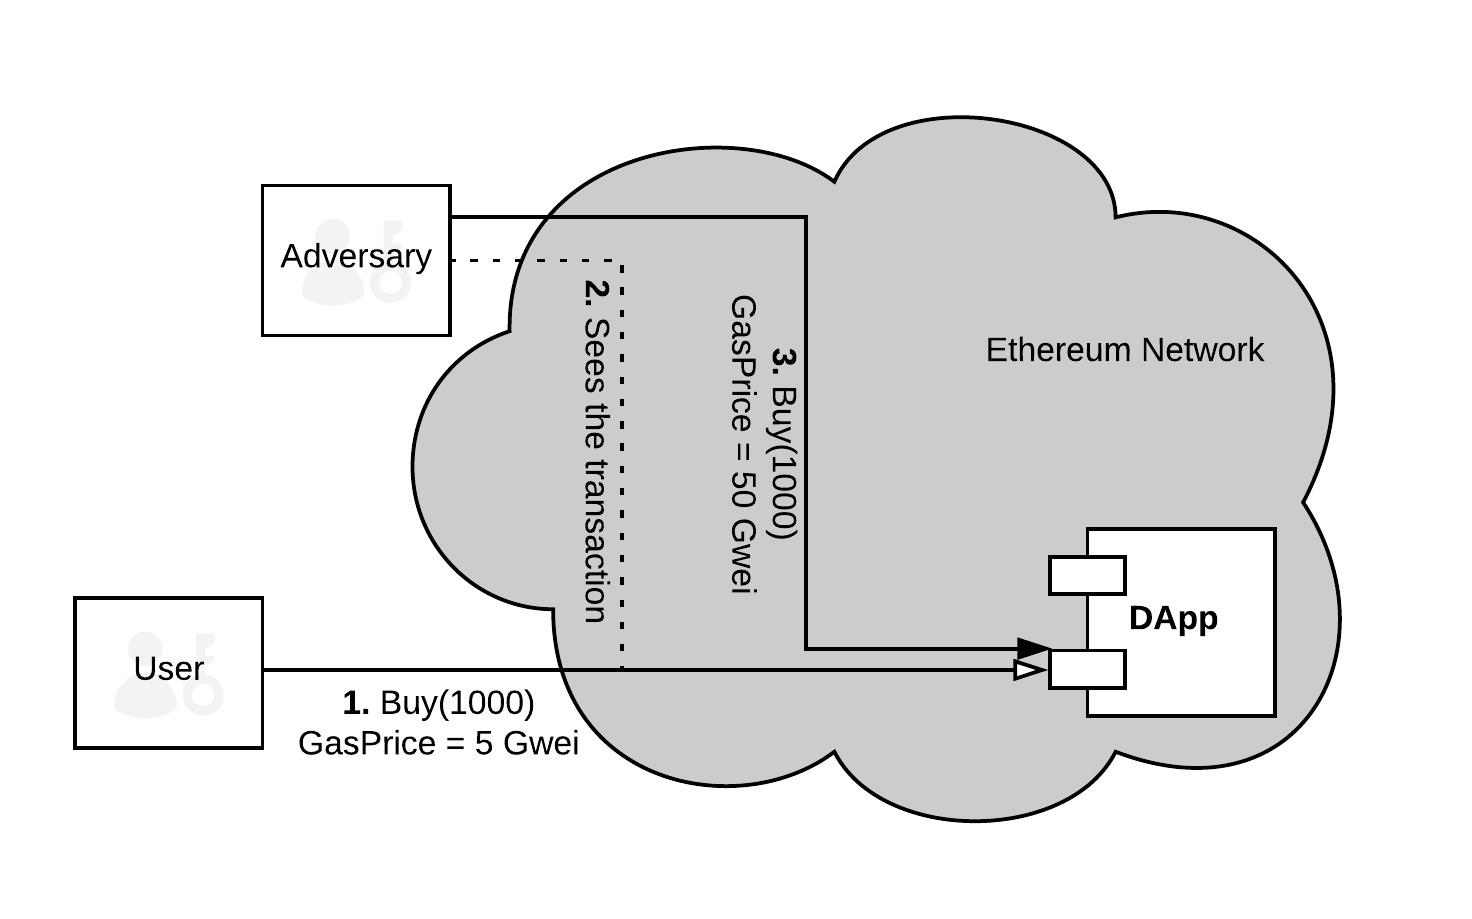
\includegraphics[width=0.7\linewidth]{figures/Regular_frontrunning.png}
\caption{The Adversary up on seeing the Buy order, sends his own buy order with higher gas to front-run the first order. \label{fig:RegularFrontrunning}} 
\end{figure}
%https://www.lucidchart.com/invitations/accept/f8ca2662-5269-425d-9deb-deb14af2aac7

\subsubsection{Miners} \label{minersfrontrunning}
Blockchain miners are the only parties who can decide on the order of transactions within a block they mine, they can easily intercept and reorder the transactions in their blocks, this in case of malicious reordering is known as \textbf{transaction reordering} attack. For example in an Ethereum based application, a miner learns about the pending \textit{buy} transaction of 1000 units of a token\ie TKN, presumably if this transaction goes through, it causes the price of the purchased token to increase. So the dishonest miner can step in front of this transaction and place his own buy order ahead. He would simply create his \textit{buy} of 1000 TKN and include it in front of the previous \textit{buy} transaction in the block he mines. Doing so, he would receive a better rate than other network users, and afterwards can sell the assets he has bought and gain a price advantage. It should be noted that miners can only front-run transactions within the blocks they happen to mine. They could do this also by not broadcasting their own transactions to the network before including it in the block, this makes the miners to be less noticeable to the network when front-running.
Another example here is in the case of decentral exchanges and order cancellation. Every exchange should have the functionality to cancel the orders, especially for a volatile market. In this case, when user decides that her order is not profitable anymore, she would send a cancelation transaction. Here the miner sees the cancelation transaction and puts his own transaction to fill that order in front of the cancellation transaction --transaction reordering--, potentially profiting from the order. He can also include the canceled transaction in the block to collect the full gas limit used by the cancel transaction~\cite{CostofDecentralization:online}, see figure~\ref{fig:MinerFrontrunning}. Front-running can also occur in non-financial smart contracts. As an example, smart contract which adds all the participants to a party invite list, could only be closed by the smart contract owner. In this case when the owner sends the transaction to close the list, a miner can include his own list of participants before the close transaction in the block he mines. This is an issue with the design of the smart contracts and is known as transaction-ordering dependence vulnerability~\cite{luu2016making}. 

\begin{figure}[h]
\centering
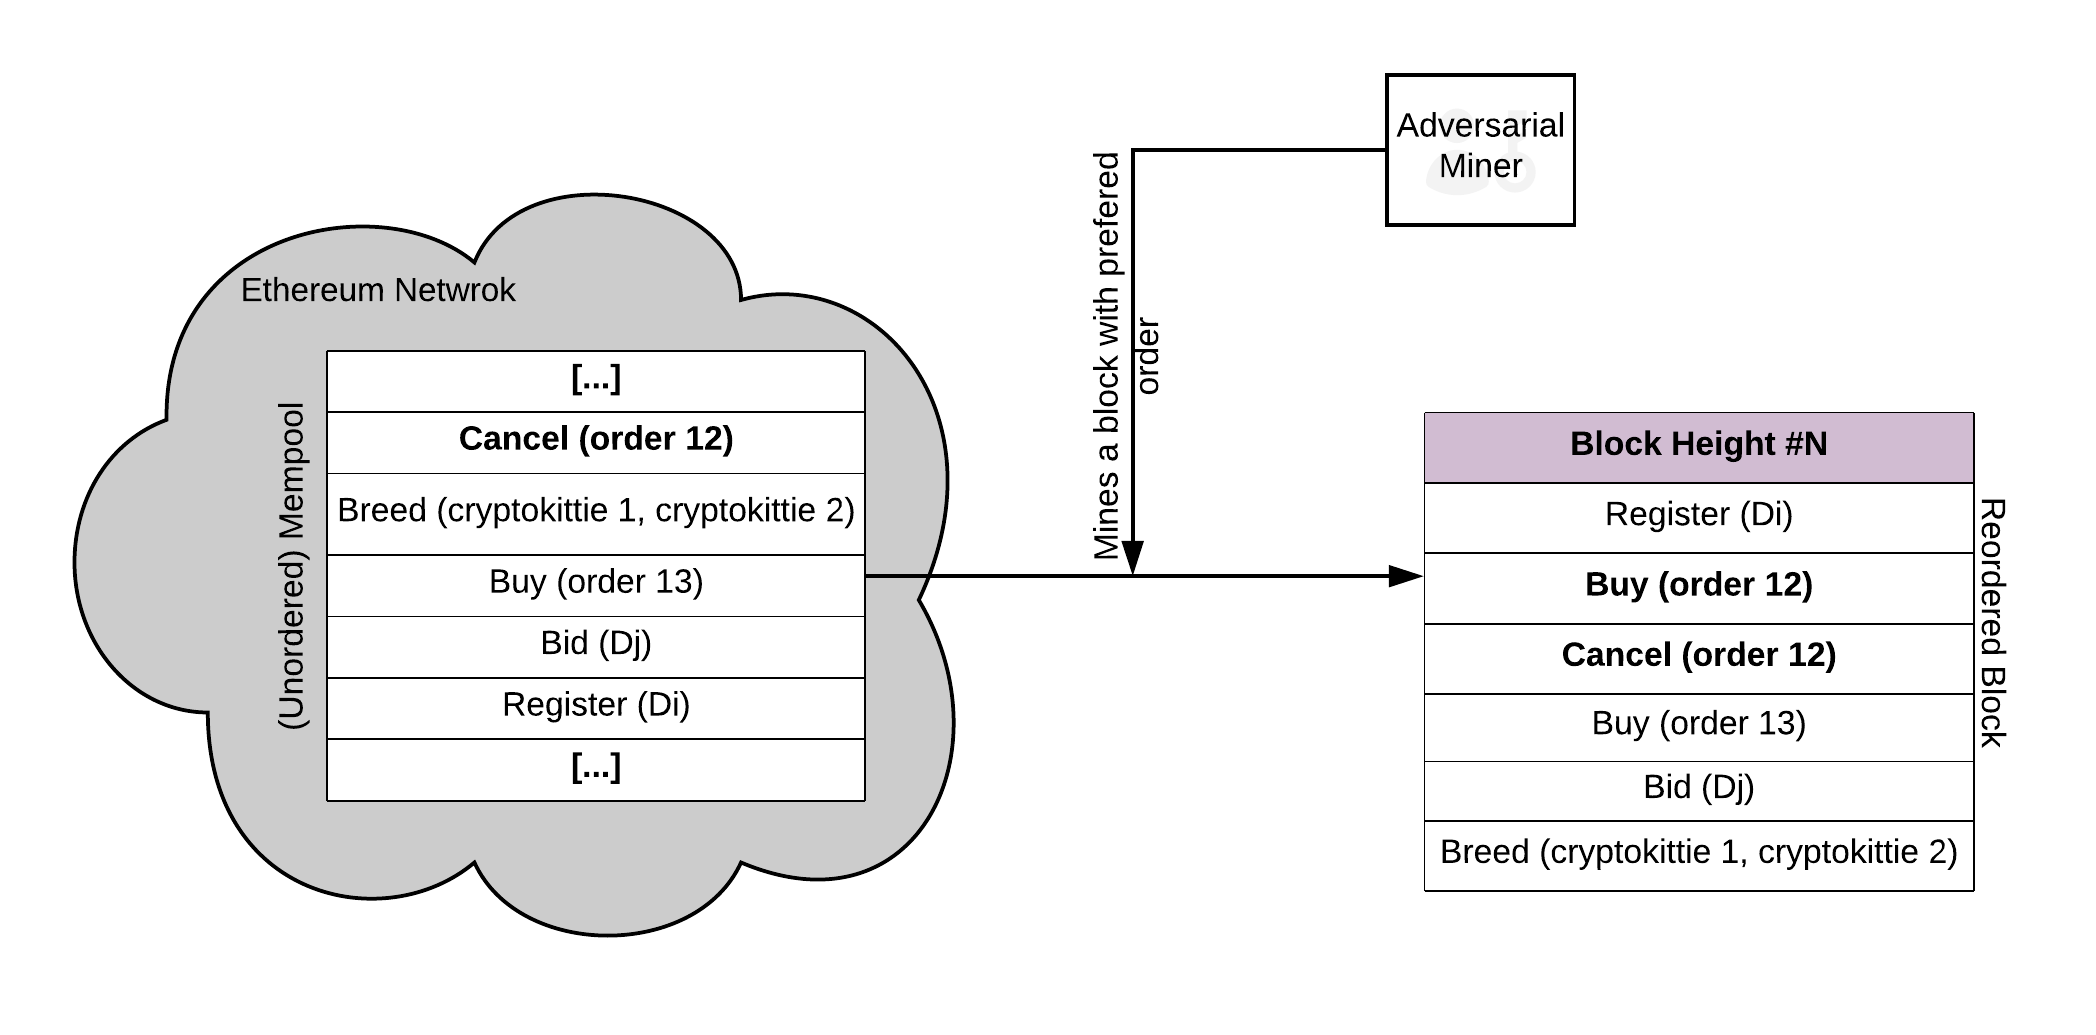
\includegraphics[width=0.7\linewidth]{figures/Miner_reorder_frontrun.png}
\caption{The adversarial miner can monitor the Ethereum mempool for decentral exchange cancel orders and upon seeing the cancellation transaction, he puts his buy order prior to the cancel transaction. Doing so, the miner can profit from the underlying trade and also get the gas included in the cancel transaction. \label{fig:MinerFrontrunning}} 
\end{figure}
%https://www.lucidchart.com/invitations/accept/c8768786-4a3f-4c78-b3c8-aa04a6b81d06


%______________________________________________________________%

\section{Cases of Front-running in DApps}  

As mentioned in the Section~\ref{sec:intro}, for the purpose of this research we retrieved the top 25 DApps based on recent user activities from \texttt{DAppradar.com}\footnote{List of decentralized applications \url{https://dappradar.com/dapps}} in the first week of September 2018. We then categorize these applications into 4 principal groups of decentral applications (see Table~\ref{tab:top25dapps}). In this section, we take a deep look into one or two decentral applications from each category and pinpoint the technical details of front-running issue on each case. Although, no ICOs were spotted in the list at the time it was retrieved, we will thoroughly discuss our analysis on how ICOs are highly vulnerable to front-running activities (see Section~\ref{sec:ICOsfrontrunning}).

% !TEX root = ../main.tex

% ------------------------------------------------------------------------------------------------------------------------------------------------%
% Top 25 Dapps Table:%

\begin{table}[t]
\centering
\scriptsize
\begin{tabular}{|c|l|}

\hline
\textbf{DApp Category}    										& \textbf{Names (Ranking)} \\  \hline
\multirow{6}{*}{Exchanges} 										& IDEX (1) \\ 
															& \textbf{ForkDelta, EtherDelta} (2) \\
															& \textbf{Bancor} (7) \\
															& The Token Store (13) \\
															& LocalEthereum (14) \\
															& Kyber (22) \\ 
															& \textbf{0x Protocol} (23) \\ \hline

\multirow{9}{*}{\shortstack{Crypto-Collectible \\ Games \\ (ERC 721)}}		& \textbf{CryptoKitties} (3) \\  
															& Ethermon (4)\\
															& Cryptogirl (9)\\
															& Gods Unchained TCG (12)\\
															& Blockchain Cuties (15)\\
															& ETH.TOWN! (16)\\
															& 0xUniverse (18)\\
															& MLBCrypto Baseball (19)\\
															& HyperDragons (25)\\ \hline

					
\multirow{8}{*}{Gambling}											& \textbf{Fomo3D} (5) \\  
															& DailyDivs (6) \\																								& PoWH 3D (8)	 \\ 
															& FomoWar (10) \\
															& FairDapp (11)\\
															& Zethr (17) \\
															& dice2.win (20) \\ 
															& Ether Shrimp Farm (21) \\  \hline	

							
\multirow{1}{*}{Name Services}									& \textbf{Ethereum Name Service} (24)  \\  \hline	


\end{tabular}
\caption{\footnotesize{Top 25 DApps based on recent user activity from \texttt{DAppRadar.com} on September 4th, 2018. We discuss the DApps that are in bold.}\label{tab:top25DApps}}
\end{table}

%TODO: mention the ones in italic are the ones we talk about
% ------------------------------------------------------------------------------------------------------------------------------------------------%

%______________________________________________________________%
\subsection{Markets and Exchanges.} \label{sec:frontrunningExchanges}

% talk about velocity that seems to be not front-runnable but because of of the liquidity pool limitation, there can be an order that consumes the last chunk of liquidity "edge case" , to front run others and make their "option calls" fail

%Tragedy of the commons

Exchanges such as EtherDelta\footnote{also known as ForkDelta for the UI \url{https://forkdelta.app/}}, are closest implementation to decentral exchanges, however their order books are stored on a central server they control and shown on their user interface (website). Other than the fact that they can re-order or censor the orders on their servers, there are other risks of front-running nature in these designs. Similarly 0xProtocol~\cite{warren20170x} uses \textit{Relayers} which act as the orderbook holders and are not prune to cheating. One main issue with these designs is the \textit{cancellation grief}. Although the orderbooks are not in the smart contract, in order to prevent denial of service attacks, user needs to send a transaction to cancel her order. In this case, when an adversarial actor sees the cancellation transaction, he sends a fill order transactions with higher gasPrice to get in front of the cancellation order and take the order before it is cancelled. As mentioned in ~\ref{minersfrontrunning}, miners are in a better position to perform such attack. 

% can we talk about Velocity here? ~\cite{eskandari2017feasibility} As the smart contract is the entity that acts as the market maker on regular cases with high liquidity front-running of the option calls do not result in any advantages, however, in the case of low balance of smart contracts pool of funds, the front-runner can front-run others to use up the remaining of the funds and make the rest of the option calls fail. 

Bancor is another Ethereum-based application that allows users to exchange their tokens without any counter-party risk. This protocol aims to solve the cryptocurrency liquidity issue by introducing \textit{Smart Tokens}~\cite{hertzog2017bancor}-- ERC20 compatible tokens with a built-in liquidity mechanism that are always available to users. ERC20 is the interface standard for implementing tokens on top of Ethereum~\cite{erc20}. Smart Tokens can be bought and sold through the users smart contract at an automatically calculated price which displays supply and demand. Doing so, Bancor protocol provides continuous liquidity for digital assets without relying on an order book as there is no requirement to match sellers and buyers.
Implemented on the Ethereum blockchain, when transactions are broadcast to the network, they sit in a pending transaction pool known as \textit{mempool} waiting for the miners to mine them. Since Bancor handles all the trades and exchanges on the Ethereum blockchain (unlike other existing decentralized exchanges), these transactions are all visible to the public for some time before being included within a block. This leaves this blockchain-based decentralized exchange vulnerable to the blockchain race condition attack as attackers are given enough time to front-run other transactions and gain favourable profits~\cite{BancorIs7:online}. Researchers have shown and implemented proof of concept code to front-run Banco as a regular non-miner user~\cite{NewTab13:online}.

%______________________________________________________________%
\subsection{Name Services.}

Front-running can also occur within non-financial blockchain applications such as naming systems. Recently, many blockchain-based domain registrars have been designed and implemented to eliminate the role of central parties \ie domain name system (DNS) which itself introduced single point of failures to the entire web. Ethereum Name Service (ENS)\footnote{\url{https://ens.domains/}}, is the most popular decentral naming service that uses a sealed auction to facilitate the procedures of purchasing new \texttt{.eth} domain names. Although sealed auction method is used in ENS implementation, the normal work flow uses \textit{startAuctionsAndBid()} with the deposit equal or higher than the bid, this information leakage could be used to front-run the transaction with the same bid amount or slightly higher to out bid the initial sealed bid. By doing so the front-runner invalidates the original bid and hence registers the domain name himself. Ghazal is another Ethereum-based naming system that allows users to register \texttt{.ghazal} domain names and bind certificates to those names~\cite{moosavighazal}.  As Ghazal is using a registration method in plain text, it is susceptible to front-running. 
Note that front-running domain names has been a subject of discussion outside the context of blockchian applications before~\cite{sac022en33:online}. Domain name registrars can steal available domain names upon seeing a query from an interested user for the availability of the domain. In this case, the registrar can register the domain name ahead and sell it back to the user for a higher price.
%______________________________________________________________%
\subsection{Crypto-Collectibles Games.}

Crypto-Collectibles, also known as \textit{ERC-721 Non-Fungible Token Standard}~\cite{erc721}, are one of the applications of Ethereum blockchain. Cryptokitties are known to be one of the first and the most popular use cases of ERC721 tokens~\cite{cryptokitties}. Their market cap reached more than 6 million dollars in the first few months their launch, however declined soon after. Crypto-Collectibles, are similar to ERC-20 tokens and can be listed on exchanges. Most of the front-running issues applied to the exchanges also apply to DApps using ERC-721 tokens. \\

As an example Cryptokitties can be bred, bought or sold through the main interface\footnote{Cryptokitties website \url{https://www.cryptokitties.co/}}. %see Figure~\ref{fig:cryptokittie}.
To buy a cryptokittie, user sends a bid transaction \textit{bid(uint256 \_tokenId)} containing the cryptokittties ID which can be found either on their website or on the ERC721 token smart contract. This is similar to open auctions, bid value and the object bidding on is visible to the network and any user could be easily front-run by sending the same transaction with higher gasPrice to replace the initial bidder. 
% https://etherscan.io/tx/0x62a76b7e345e8abd463487d0348c118a9314b197024e090fee7b1fbce434da40

%Possibly remove this figure due to page limit
\begin{figure}[h]
\centering
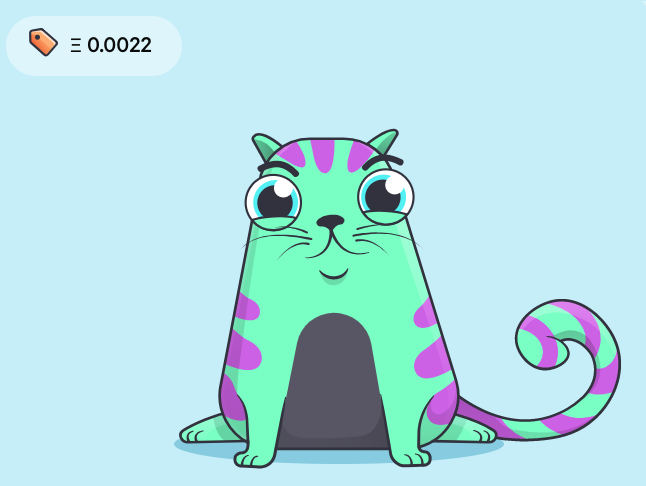
\includegraphics[width=0.3\linewidth]{figures/cryptokittie842912.png}
\caption{ Cryptokitty Number 842912 \label{fig:cryptokittie}}
\end{figure}

%______________________________________________________________%

\subsection{Gambling.} 

Due to deterministic nature of blockchains, running gambling games based on randomness is close to impossible. There had been attempts to use block headers or such as the seed to randomness but almost all have failed as every data accessible to the smart contract at the time of execution, is also accessible to other smart contracts and they could predict the output on the run, thus prone to front-running and miner\'s manipulation. Many infamous gambling games are now running on Ethereum network and front-running them requires a level of sophistication and knowledge of the internal of the games and Ethereum.\\
One of the most popular smart contracts on Ethereum blockchain belongs to a controversial gambling game named \texttt{Fomo3d}, also known as \textit{Exit Scam}\footnote{\url{https://exitscam.me/play}}. The aim of this game is to be the last person purchasing the key when the timer goes to zero in which every ticket purchase increases the timer by 30 seconds. It was believed that because of the nature of the game, it will never end, however on August 22, 2018 the first round of the game ended and the winner taking 10,469 Ether\footnote{First winner of Fomo3D, won 10,469 Ether \url{ https://etherscan.io/tx/0xe08a519c03cb0aed0e04b33104112d65fa1d3a48cd3aeab65f047b2abce9d508}}, equivalent to 2.1 Million dollars on the time of writing. 
It is believed that the winner, used a sophisticated approach to finish last~\cite{fomo3dhacker}, we call this approach \textit{Denial-of-service Front-running}. The winner deployed a few high gas consumption smart contracts prior to the win, when the timer of the game reached about 3 minutes, the winner bought 1 ticket and sent multiple high gasPrice transactions to aforementioned smart contracts to lure the miners to mine these highly profitable transactions. For a DoS front-running to work, attacker floods the network with high gasPrice transactions to prevent other transactions to go through. Luckily enough the winner was able to congest the network in a way that no other ticket purchases were mined in the 3 minutes window and the miners were prioritizing the high gasPriced transactions over other transactions. All the details mentioned here are drawn from the transaction history on the blockchain and unless otherwise proven seem to be the way the winner acted to win the pot. 
%probably needs more work to be good enough. more resources will be out in the coming days !

%______________________________________________________________%


\section{Cases of Front-running in ICOs}  \label{sec:ICOsfrontrunning}

There has been more than 3000 ICOs on Ethereum alone, estimated to exceed 75 billion dollars in the first half of 2018~\cite{zetzsche2018ico}. On our DApp samples there was not ICOs mainly because they tend to run for a short time with high number of participant and in the time of writing no ICOs have reached the top 25 DApps of \texttt{DAppradar.com}. Needless to say the importance of ICOs as an application of blockchain requires more in-depth analysis of front-running on these DApps. %ICOs due to the defined cap, are similar to our analogy of a queue line, people would line up to get in and there's a opportunity to front-run. 
Here we focus on one ICO that our preliminary research showed that there might be a front-running attack going on. There is no doubt that similar behaviour could be seen on other instances of ICOs or similar DApps if investigated.

\subsection{\textit{Status.im} ICO}
As discussed in~\ref{sec:Front Running on the Blockchains}, capped ICOs are considerable applications to be investigated in terms of the front-running attacks, \textit{Status.im} ICO is such application. In June 2017, \textit{Status.im}~\cite{statuswhitepaper} started its ICO and reached the defined cap within 3 hours, resulting in close to 300,000 Ether of funds. In order to prevent few large investments to buy up all the tokens and limit the amount of Ether deposited in an investment, they used a \textit{fair} token distribution method named \textit{Dynamic Ceiling} as an attempt to increase the time window for smaller investors. They implemented multiple caps --ceiling-- in which, each had a maximum amount that could be deposited in. In this case, every deposit was checked by the smart contract and the exceeding amount was refunded to the sender while the accepted amount was sent to their multi-signature wallet address~\cite{statusicoanalysis}. 

During the time the ICO was open for participation, there were reports of Ethereum network being unusable and transactions were not confirming. Further study showed that some mining pools might have been manipulating the network for their own profit. In addition, there were many transactions sent with higher gas price to front-run other transactions, however these transactions were failing due to the restriction in the ICO smart contract to reject any transactions with higher than 50 \textit{GWei} gas price (as an attempt to prevent the known front-running behaviour).

\begin{figure}[h]
\centering
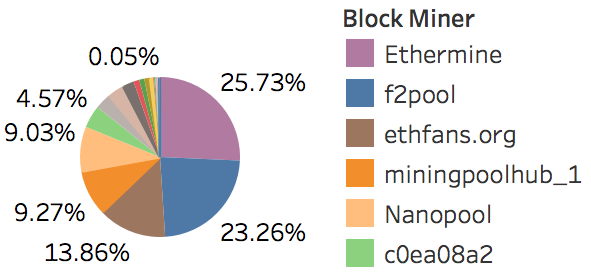
\includegraphics[width=0.5\linewidth]{figures/Mining_pool_ratio.png}
\caption{The percentage of Ethereum blocks mined between block 3903900 and 3908029, this is the time frame in which Status.im ICO was running. This percentage roughly shows the hashing power ratio each miner had at that time. \label{fig:mining_pool_ratio}} % IS THIS STATEMENT CORRECT?
\end{figure}

\subsection{Data Collection and Analysis}
According to the analysis we carried out, it was discovered that the F2Pool, an Ethereum mining pool that had around 23\% of the mining hash rate at the time (Figure ~\ref{fig:mining_pool_ratio}), sent 100 Ether to 30 new Ethereum addresses before Status.im ICO started. On the time the ICO was opened for participation, F2Pool constructed 31 transactions to the ICO token sale smart contract from the addresses they controlled --without broadcasting these transactions to the network-- and used their entire mining power to mine their own transactions and also potentially failing high gas price transactions.

Ethereum blockchain contains all transaction ever made on Ethereum, however, it is not easy to see the behavior of the participants and miners solely using the default clients nor online blockchain explorers. In order to get the required data, Ethereum blockchain data should be converted to a queryable format. For this case study, we used open source projects such as Go Ethereum implementation\footnote{Official Go implementation of the Ethereum protocol\url{https://github.com/ethereum/go-ethereum}} for the full node, python script for extracting, transforming and loading ethereum blocks, named \texttt{ethereum-etl}~\cite{ethereumetl} and Google BigQuery\footnote{A fast, highly scalable, cost-effective, and fully managed cloud data warehouse for analytics \url{https://cloud.google.com/bigquery/}}. Using this software stack, we were able to query for all the transactions and blocks within the window of Status.im ICO for further analysis which was mainly done by data analysis tool \texttt{Tableau}\footnote{Tableau is a data visualization software that is used for data science and business intelligence.\url{https://www.tableau.com/}}. A copy of this dataset and the initial findings can be found in our Github repository\footnote{\url{github.com / ANONYMOUS}}. 


As shown in Figure~\ref{fig:Transactions_miners_while_status_ico_cut}, most of the top miners in the mentioned time frame, have mined almost the same number of failed and successful transactions which were directed toward Status.im token sale, however F2Pool's transactions indicate their successful transactions were equivalent to 10\% of the failed transactions, hence maximizing the mining rewards, on gas, while censoring other transactions to the token sale smart contract. The terminology used here is specific to smart contract transactions on Ethereum, by \textit{``failed transaction''} we mean the transactions in which the smart contract code flow rejected and threw an exception and by \textit{``successful transaction''} we mean the transactions that went through and received tokens from the smart contract. 


\begin{figure}[h]
\centering
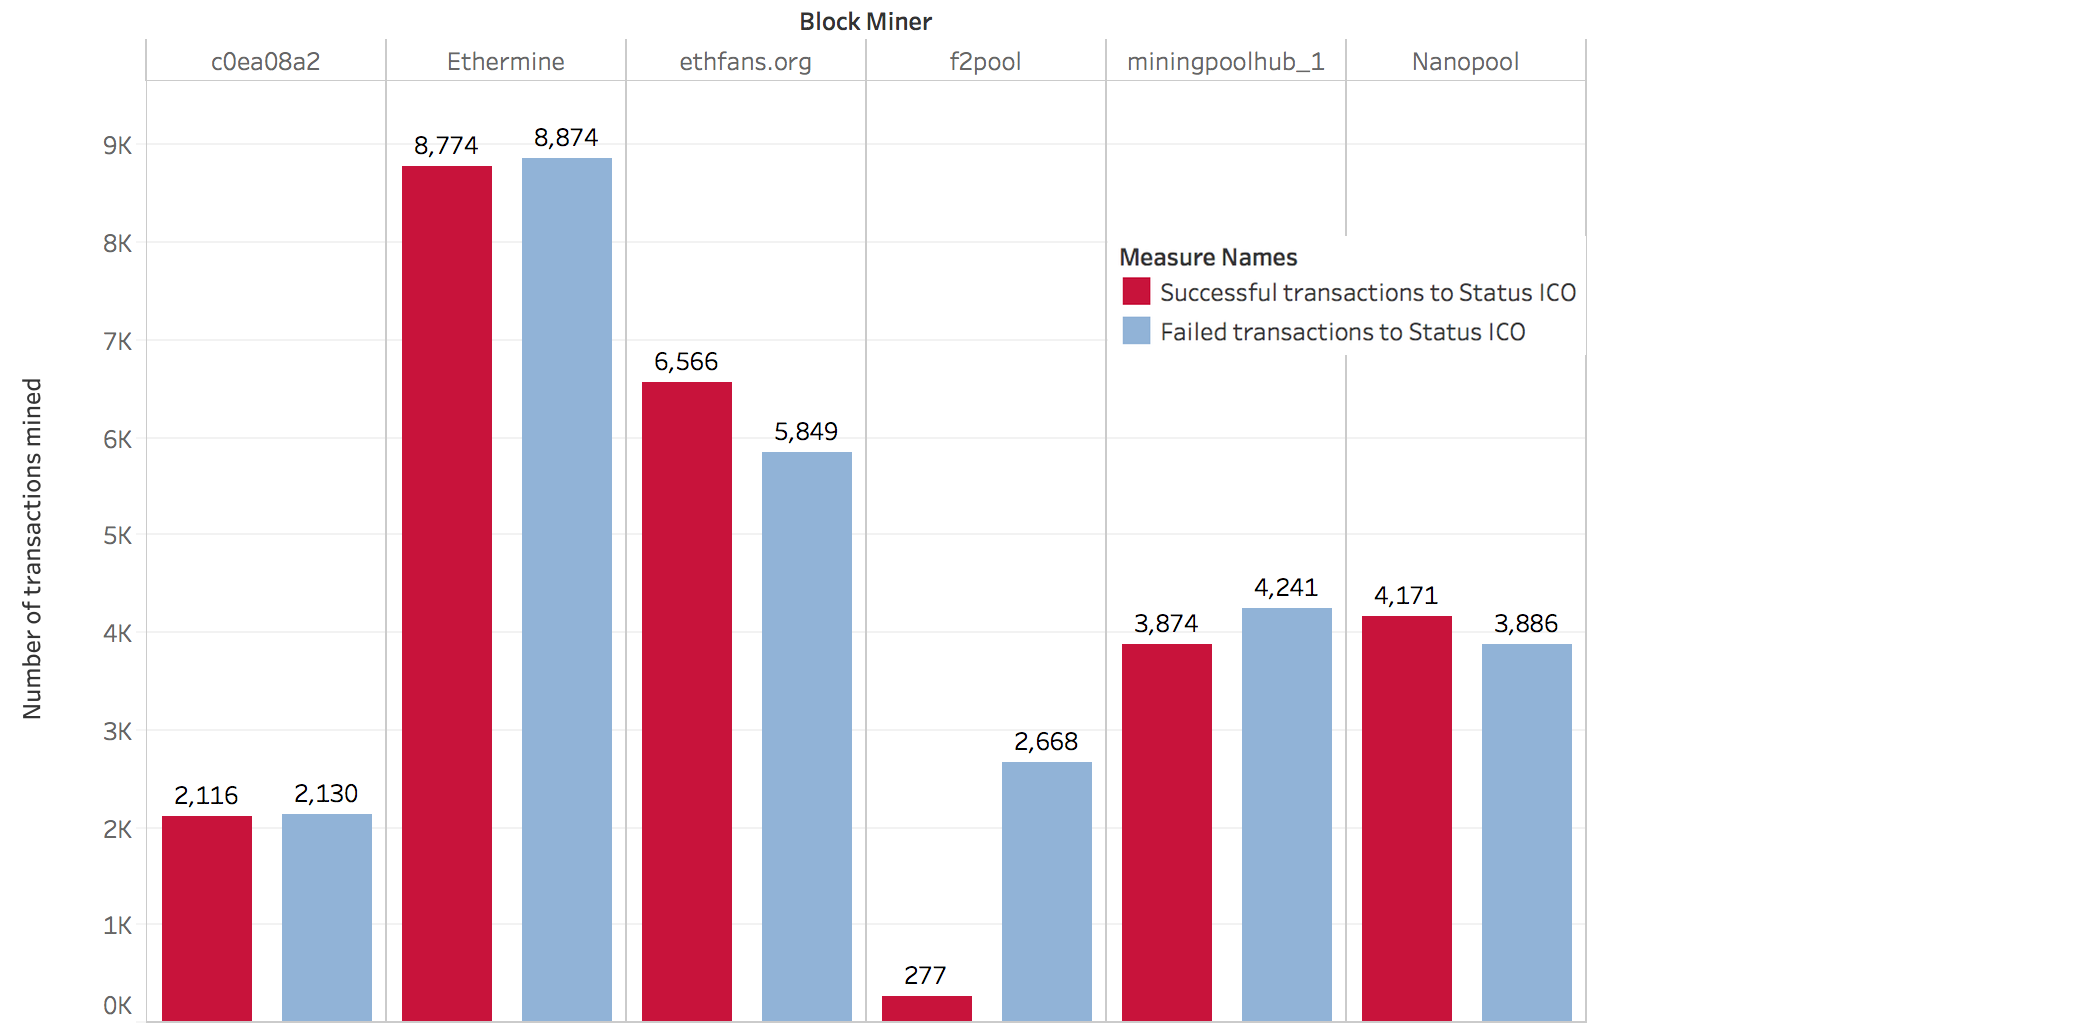
\includegraphics[width=0.7\linewidth]{figures/Transactions_miners_while_status_ico_cut_only_icotx.png}
\caption{This chart shows the miners behaviour on the time window that Status.im ICO was running. It is clear that the number of successful transactions mined by F2Pool do not follow the random homogeneous pattern of the rest of the network. \label{fig:Transactions_miners_while_status_ico_cut}} 
\end{figure}

% make pie charts for each mining pool, all non-status-ico transactions vs success-ico-transactions vs failed-ico=transactions

By tracing the transactions from these 30 addresses, we found explicit Interference of the F2Pool\footnote{F2Pool Ethereum address was identified by their mining reward deposit address \url{https://etherscan.io/address/0x61c808d82a3ac53231750dadc13c777b59310bd9}} in this scenario. As shown in Figure~\ref{fig:f2poolfront-run}, the funds deposited by F2Pool in these addresses were sent to Status.im ICO and mined by F2Pool themselves, where the dynamic ceiling algorithm refunded a portion of the deposited funds back to these addresses, these funds were sent back to F2Pool main address a few days after. 

\begin{figure}[h]
\centering
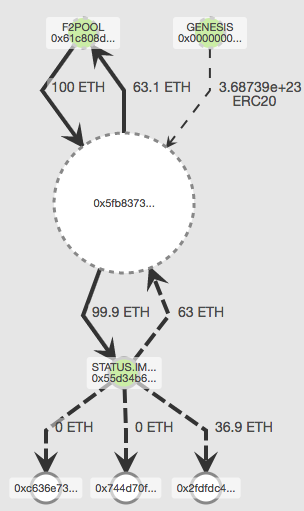
\includegraphics[width=0.7\linewidth]{figures/F2Pool_transactions_to_StatusICO_and_Refunds.png}
\caption{F2Pool prior to Status.im ICO deposited 100 Ether in multiple new Ethereum addresses. On the time of the ICO they sent these deposits to Status ICO smart contract and prioritized mining of these transactions in their mining pool, this was to overcome the dynamic ceiling algorithm of the token sale smart contract. Later on they sent the refunded Ether back to their own address. [Graph made using Blockseer.com] \label{fig:f2poolfront-run}}
\end{figure}


Although this incident does not involve transaction reordering in the blocks, it shows how miners can modify their mining software to behave in a certain way to front-run other transactions and take advantage of the monetary profit. The dataset used for this analysis can be found on our GitHub repository.\footnote{Frontrunning Status.im ICO dataset: \url{http://github.com/TODO:ANONYMOUS}}. This analysis made us wonder how many other DApps are vulnerable to front-running attack, who can front-run and what are the mitigation methods for decentral applications?

%______________________________________________________________%


\section{How to stop Front-running?} %We have the applicability of the solutions inline.

In the traditional markets, front-running is considered unethical and also illegal. In the blockchain space, the designers of the decentral applications cannot rely on the justice system for unethical behavior, and they must assume that each participant in the network acts rationally in their own self interest, the application will be operating in an adversarial environment~\cite{0xfrontrunning:online}.
A few decentral exchange projects such as \textit{EtherDelta} and \textit{0xProject}~\cite{warren20170x}, have proposed solutions for front-running, which is off-chain order books. The methods discussed within these projects prevent blockchain network participants from front running the orders as the orders are private and not known to the network and will not be broadcasted. However they are introducing third parties, \eg relayers in 0xproject, to be managing the orders with the promise not to reorder or front-run other orders. 

\emph{Traditional Front-running Prevention Methods}. There are debates in traditional markets regarding the fact that Front-running is considered to be a form of insider trading which deemed to be illegal. Traditional methods to prevent front-running mainly involves after the fact investigation and legal action against the front-runners~\cite{LexisNexisLawSuit}. As mentioned in section~\ref{traditionalFrontrunning}, educating the employees were the first step taken to prevent such issues in traditional markets, however front-running became less likely to happen mainly because of the high fine and law suits against firms whom behaved in an unethical way. Other methods such as dark pools~\cite{zhu2014dark, buti2011diving} and sealed bids~\cite{radner1989sealed} were discussed and implemented in variety of regulated trading systems. 

The traditional methods to prevent front-running does not apply to blockchain applications, as mainly they are based on central enforcement and limitations, also in case of blockchains the actors whom are front-running could be anonymous and the fear of lawsuits would not apply. \\

There are two main approaches to prevent front running, one to design a blockchain that is front-run resistant , and the other to design the application logics in a way that front running is not possible. 
%______________________________________________________________%
\subsection{Front-run Resistant Blockchain}
What does this mean to have a front-run resistant blockchain?  There are technical difficulties to achieve such solutions as there are unknown factors within such network designs (corner/edge cases). In this section, we describe the potential solutions using which, one can design and implement a decentral application that is resistant to front-running.

\subsubsection{Design Decision \#1: Fixed Transaction Ordering\newline}

One possible solution to fix current blockchains in regards to transaction reordering by miners has been proposed by da Silva~\etal~\cite{fixedordering2018silva}. This solution consists of an algorithm, known as Fixed Transaction Ordering and Admission (FTOA) algorithm, in the consensus protocol that enforces the order of the transactions. 

\subsubsection{Design Decision \#2:Privacy Preserving Blockchain\newline}

Market participants are concerned about revealing information on their past trades, purchases, income, or liquidity needs. Privacy is a basic human right, that being said, there are limitations with the functionality of a system designed to preserve full privacy. However other than past transactions, real time transactions could leak informations about the sender or the intention of the order that could lead to front-running attacks. Privacy preserving blockchains try to solve the initial issue by keeping all the details of the transactions private, in some extent~\cite{miller2017empirical, kappos2018empirical}. 
As an example, ZCash~\cite{hopwood2016zcash}, uses two distinct type of addresses, transparent addresses and shielded addresses. Transparent addresses work similar to Bitcoin transactions, fully transparent about the sender and receiver addresses, the amount and included data. However shielded addresses are private and do not leak any information, this is great for privacy but not good for smart contracts capabilities. Smart contract functionality requires verification by the miners which require to know the input, functionality and output of smart contracts to be able to determine if the transaction is valid. Albeit by using cryptographic primitives such as zero-knowledge proofs this issue could also be resolved~\cite{kosba2016hawk}. 


\subsubsection{Design Decision \#3: Dual Authoring\newline}

Loopring is an open protocol proposed by Wang~\etal to build decentralized exchanges~\cite{wang2018loopring}. This protocol operates a hybrid model with off-chain order management and communication and merely the order matching takes place on the chain. To achieve high liquidity and price improvement, Loopring orders are grouped in \emph{ring orders}. After the required signatures are provided by a miner and owner of the order, see Figure~\ref{fig:vulnerable_loopring}, the ring miner sends the \emph{submitRing transaction} to the Loopring Smart Contract (LPSC) for verification and settlement. While the \emph{submitRing transaction} sits unconfirmed in the mempool, any front-runner can create a copy of this transaction with his address instead of the ring miner's address and then sign the hash of the ring using his own private key. By paying a higher gasPrice, block miners choose the front-runner's transaction instead of the original \emph{submitRing transaction}. However, Loopring's team solves this issue using the \emph{dual-authoring} scheme in the new version of the Loopring protocol. This solution sets two levels of authorization for orders - one for settlement, and one for order matching. As it can be seen in Figure~\ref{fig:not_vulnerable_loopring}, each owner of any order generates a pair of public key (auth-address) and private key (auth-key), which are different from his address and its corresponding private key. These auth-keys are used to sign the hash of the ring and will further prevent anyone from regenerating the same \emph{submitRing transaction}. The reason is that the auth-keys are only known to the miner of the ring as they are not part of on-chain transaction. Doing so, it is assured that (i) the orders are not modified (because they are signed using the owner's private key), (ii) no other miner can mine the ring (because the miner's address is signed using his private key), and no user can front-run the \emph{submitRing transaction} (because other users do not have access to the auth-keys and hence are not able to generate new transactions with auth-keys signatures on them).

\begin{figure}[h]
\centering
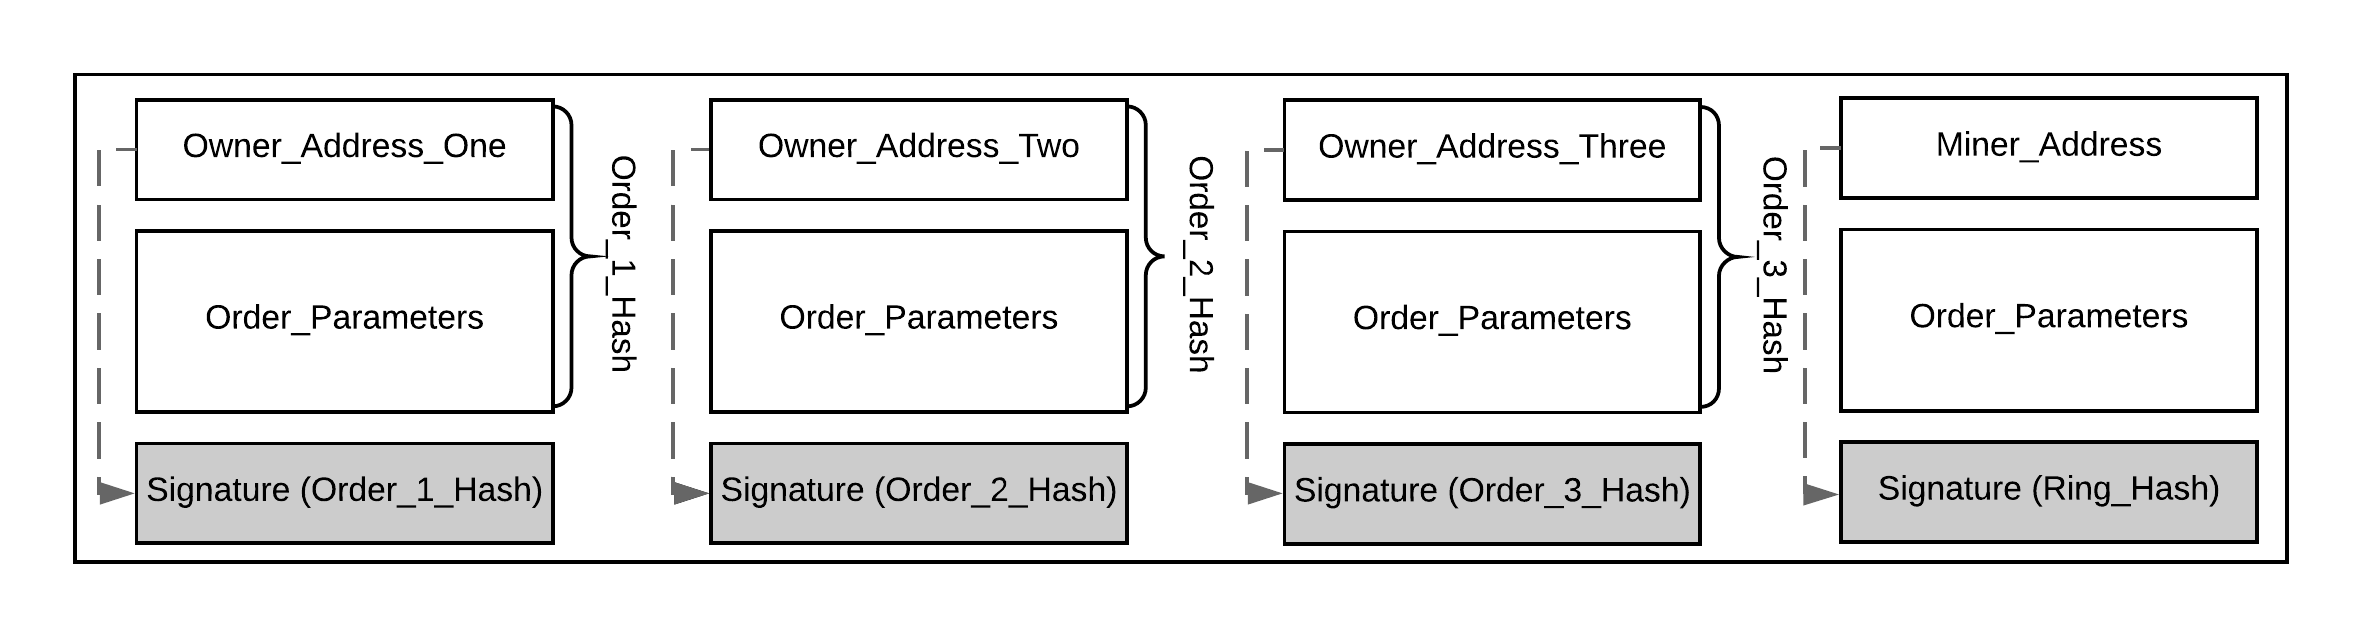
\includegraphics[width=0.7\linewidth]{figures/Vulnerable_Loopring.png}
\caption{\emph{submitRing} Transaction in the old version of the Loopring protocol. Any user can regenerate this transaction by replacing the miner's address with his address and signing the hash of the ring using his private key. \label{fig:vulnerable_loopring}}
\end{figure}
%https://www.lucidchart.com/invitations/accept/33d38ce9-4660-4743-806d-45c72f7e8393
\begin{figure}[h]
\centering
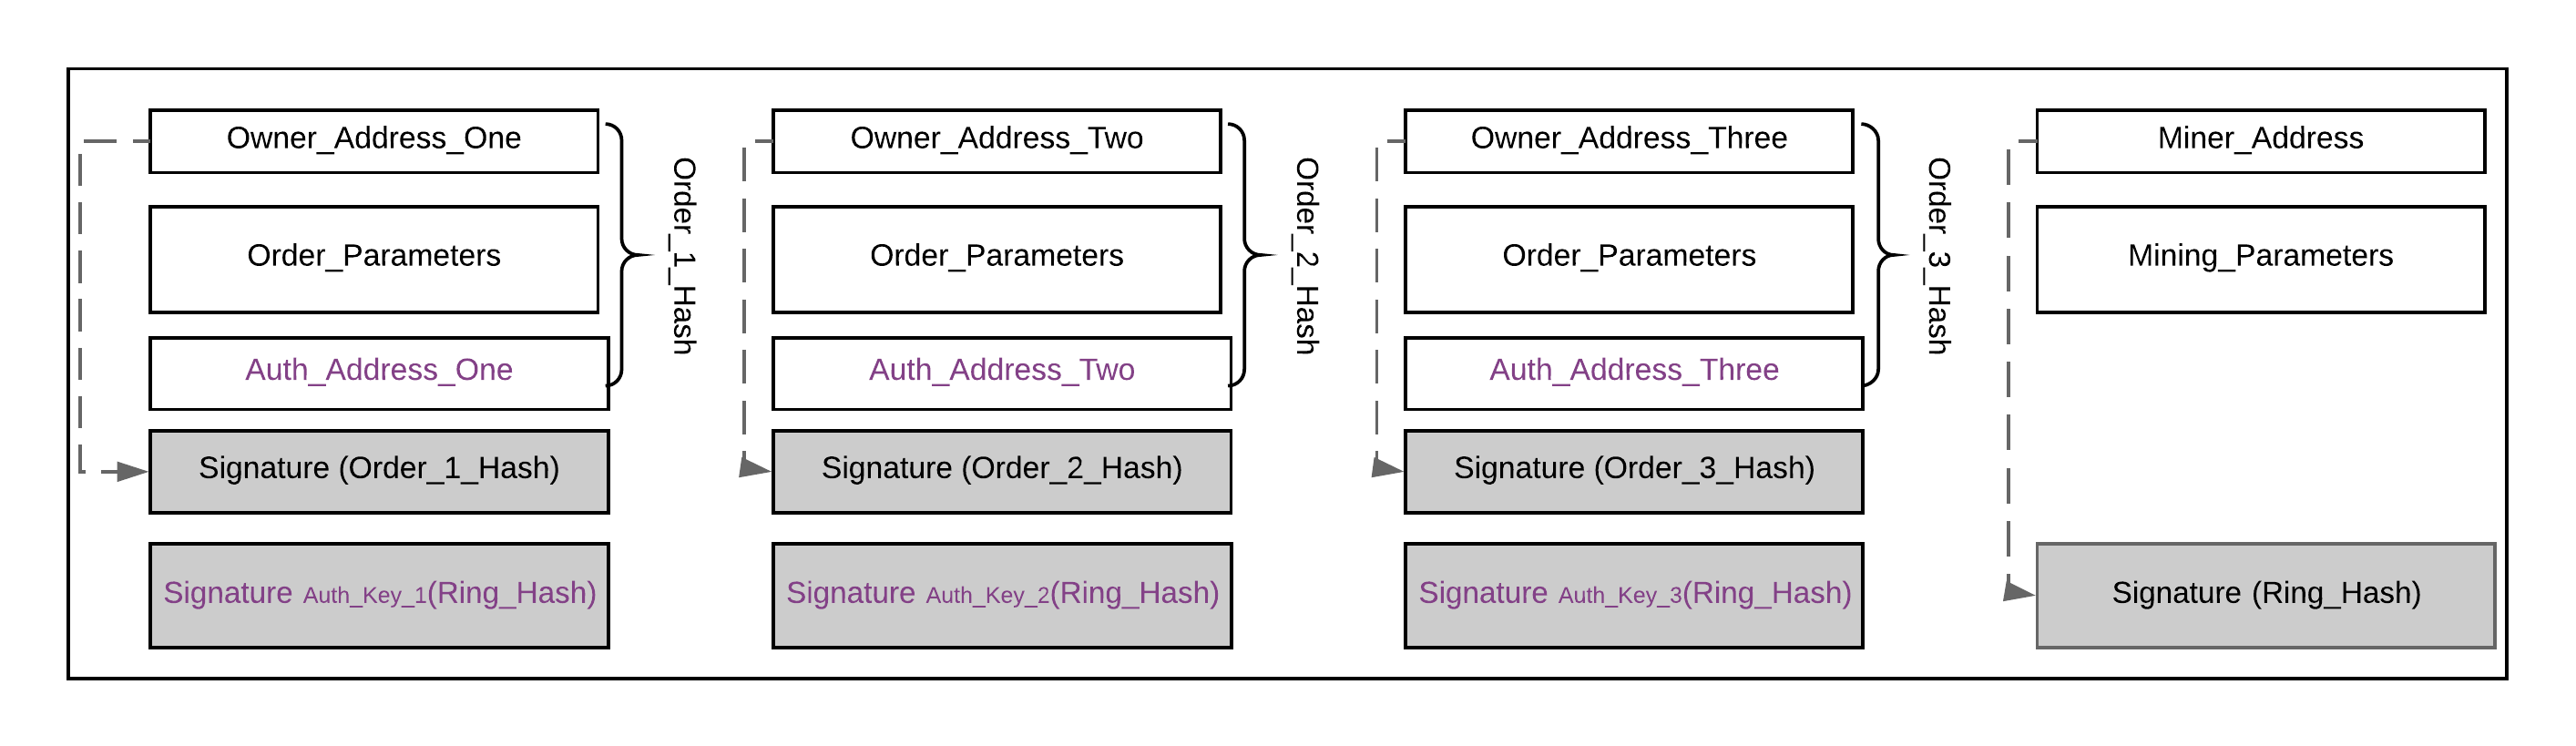
\includegraphics[width=0.7\linewidth]{figures/Dual_Authoring_Loopring.png}
\caption{\emph{submitRing} Transaction in the new version of the Loopring protocol. Other users cannnot regenerate this transaction as they do not access auth-keys and hence are not able to create the signatures. \label{fig:not_vulnerable_loopring}}
\end{figure}
%https://www.lucidchart.com/invitations/accept/8dee869c-482c-433f-a901-8d041a1dc526
%______________________________________________________________%
\subsection{Application Design to Prevent Front-running}

Another method to prevent front-running activities is to design the applications, whether they are decentralized (Dapps) or centralized, in such a way that no information would be available to the malicious parties to enable them to front-run the other users.
Followings discuss the two techniques which can be used by the Apps/DApps developers while designing the systems to prevent front-running activities.

\subsubsection{Design Decision \#1: Commitment Scheme\newline} \label{CommitmentScheme} %talk about the drawbacks of this scheme: eg: you may forget to reveal. 
Commitment scheme is a cryptographic primitive that enables one to commit to a value --binding-- (\eg statement, document, data, \etc) while keeping it a secret and reveal the committed value on a later time~\cite{brassard1988minimum}. Commitment scheme is a robust method to prevent information leakage from the sensitive transactions. This could be done by simply broadcasting the hash value of the committed data and later on revealing the values that would be hashed to the committed hash, see Figure~\ref{fig:commitReveal}. 
In the case of decentral exchanges, user can send a commit transaction which will be cryptic to network participants but will act as a placeholder in the queue for the user, after the transaction is mined, user sends reveal transaction revealing the order details which will be executed in a fair order. Depending on the Dapp design, either the order is collateralized, which means the commitment transaction includes the funds required for fulfilling the order, which will leak some information about the order, or is not collateralized and opens up the possibility of user never revealing the commitment, which will be considered as a DoS attack. 
Another use of such commitment scheme, is in decentralized naming systems, such as Namecoin, Ethereum Name Service (ENS) or Ghazal. In this case, a user sends a commit transaction, which commits to the name hash, similar to a sealed bid. Once the transaction is confirmed and the grace period is over, user sends a reveal transaction revealing the bid and also the details of the requested domain~\cite{kalodner2015empirical}. Using this scheme, one is able to hide information from the adversarial parties in the system and prevent them from front-running. Similar approach applies to on-chain voting as well ~\cite{adChainPLCRVoting}, using sealed votes, voters can make sure their votes are hidden until a later date, however their participation and weight of the vote are publicly known. 
Other than the collateralization issue for the commit and reveal scheme, another obvious issue is the participatory factor. For anyone watching the DApp address, there will be a direct transaction from the user to the DApp address, It will be obvious that a specific address has participated in the auction or the DApp using a commit and reveal scheme, but the details are hidden through the scheme. Both these issues, albeit hiding the details of the order and preventing direct front-running, leak information to other participants which could lead to more sophisticated front-running attacks depending on the application design. On the other note, these method has some drawbacks, the user experience is not smooth and one might forget to reveal the committed transaction. In ENS commit-reveal process, if one forgets to reveal on the reveal phase, the committed funds are burnt and inaccessible there after. Also this scheme means two transaction are required for a functionality which is makes it more expensive to run.

\begin{figure}[h]
\centering
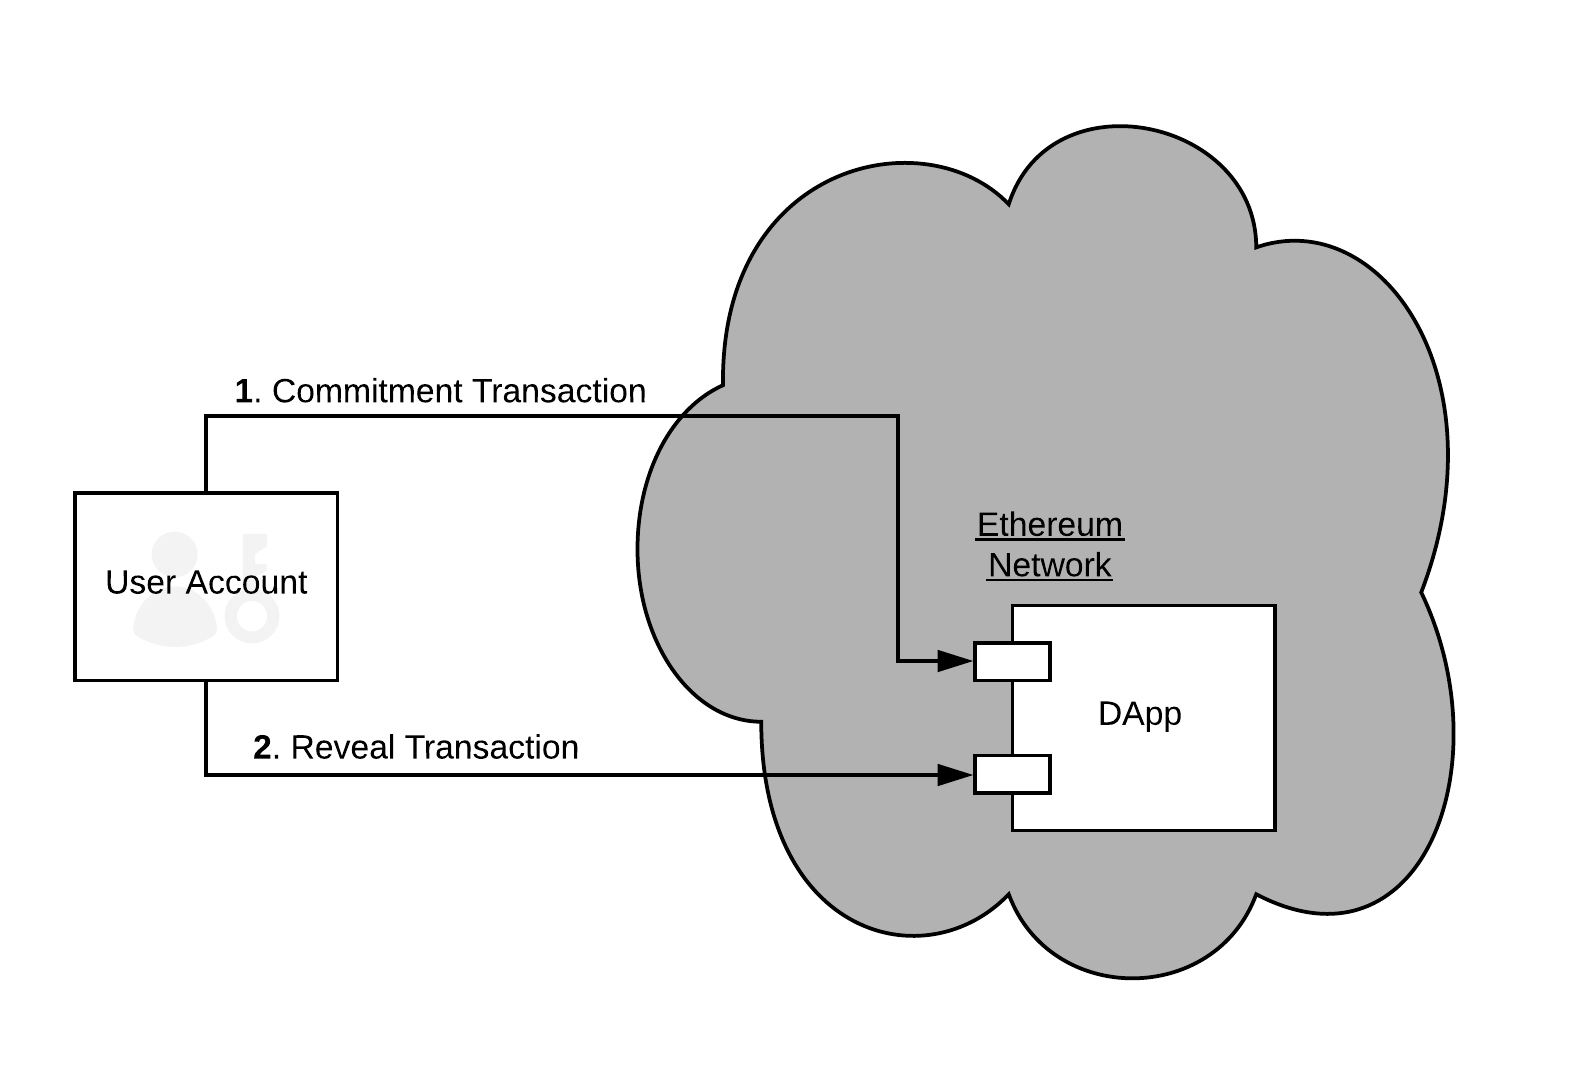
\includegraphics[width=0.5\linewidth]{figures/commit-reveal.png}
\caption{ Commit and Reveal. User sends a commitment transaction with the hash of the data, After the commitment period is over, user sends her reveal transaction to the DApp revealing the information that matches the commitment. \label{fig:commitReveal}}
\end{figure}
%https://www.lucidchart.com/invitations/accept/3cd4c865-83d4-4c71-9a4a-f2e870f2db2c

\subsubsection{Design Decision \#2: Submarine Commitments\newline}\label{submarineCommits}
Submarine Commitments~\cite{breidenbach2018enter, submarinesendHD} are similar to the commitment schemes with some key differences such as hiding participatory factor and being fully collateralized. However, they could be design in other ways to suit the need of the DApp. With submarine send, it is possible to hide sender, receiver, value and data, the commitment transaction is identical to a transaction to a newly generated address. Submarine sends could be a solution for sealed-bid auctions on the blockchain to hide the existence of the bids for other participants. 

The details of how Submarine commitments work is outside the scope of this paper, however in summary, using the way Ethereum transactions are constructed and ECDSA ECRecover functionality it is possible to generate one outgoing transaction from an address in which no private key exists. By constructing a transaction from that address to the DApp and funding that address we fulfill the commitment phase and by revealing the details and broadcasting the constructed transaction we reveal the commitment ~\cite{libsubmarine}, see Figure~\ref{fig:LibSubmarine}.  Drawbacks of this scheme are similar to ~\ref{CommitmentScheme}, with an addition of two more transactions to finalize the functionality, which results in more cost and complicated user experience.


\begin{figure}[h]
\centering
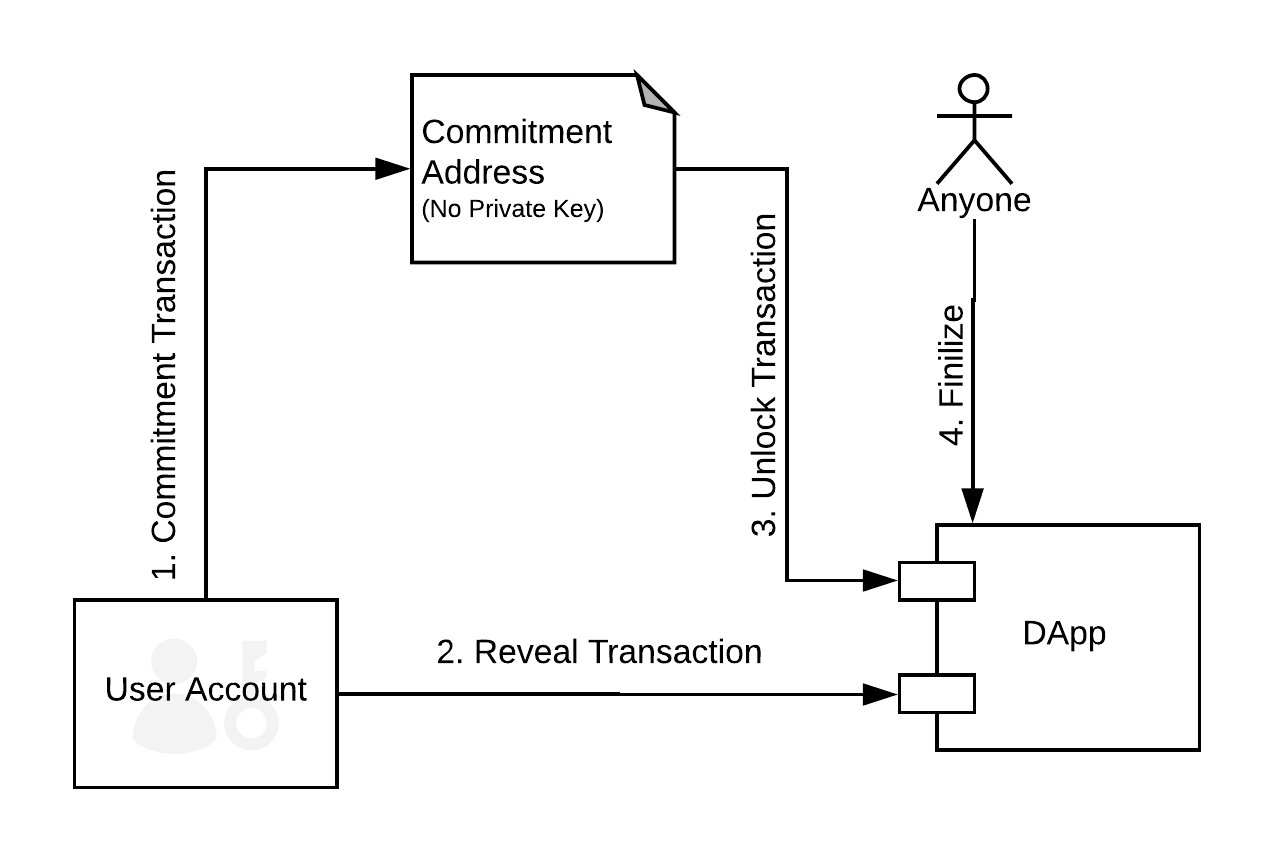
\includegraphics[width=0.5\linewidth]{figures/LibSubmarine.png}
\caption{ Submarine Send~\cite{libsubmarine}. User generates an \textit{Unlock} transaction from which the commitment address is retrieved. By funding the \textit{commitment address}, user is committed to the unlock transaction. After the commitment transaction, in the reveal phase, user sends the \textit{reveal transaction} to the DApp and then after she can broadcast the Unlock transaction to unlock the funds in the commitment address. Finally after the "Auction'' is over, anyone can call \textit{Finalize} function to finalize the process.  \label{fig:LibSubmarine}}
\end{figure}
%https://www.lucidchart.com/invitations/accept/3a259b74-1162-4fb5-8023-eb0311018295


\subsubsection{Design Decision \#3: Logic Specific Solutions\newline}
To prevent front-running, one can design the application in a way that it is not possible to be front-run:

\noindent\emph{Eliminating Time-Order Dependency:} The applications can be designed to not rely on the time for the orders to be executed. For example when designing a decentral exchange, one can use \emph{the call market design} instead of a time-sensitive order book. In a call market design, the arrival time of the orders do not matter as they are executed in batches [cite Jeremy's prediction markets paper]. 

\noindent\emph{Disincentivizing Front-running Actors:} This solution, which is economic rather than technical, is to disincentives the miners by paying them. As mentioned, the main reasons for miners to front-run the other orders is the financial gain they receive on the price improvement. However, if the application is designed in a way that the fees of the orders are sent to the miner of the block, he would have no incentive to front-run the orders as he already gains enough financial benefit from acting fairly and executing the transactions on their correct order. For example, Malinova~\cite{malinova2017market} proposes a design for a decentral exchange which uses economic models in their trading market design to make front-running expensive and more costly than profitable. 


% one solution could be to remove multiple actors, meaning that on each "play" (order), the smart contract would be the market maker. it does not matter if there are multiple similar orders. similar to PoC of Velocity~\cite{eskandari2017feasibility}. Although there are other concerns about this specific design but not for front-running.


Going back to Table~\ref{tab:top25dapps}, some DApps facilitate different methods to mitigate front-running issues. As an example LocalEthereum, an escrow-based exchange, uses challenge random values from the website to be included in the signature of the transaction (See ~\ref{code:localethereum}), hence removing any possibility of replay attack or possibility of any other address sending the similar order.

%Possibly remove this code snippet due to page limit
\begin{lstlisting}[basicstyle=\scriptsize\ttfamily,caption={Code snippet from LocalEthereum smart contract. Values V,R and S are set by LocalEtherem to have a valid signature, also the tradeHash uses buyer and seller addresses, mitigating the possibility of front-running by a third party.},label={code:localethereum},float]
    function createEscrow(bytes16 _tradeID, address _seller, address _buyer, uint256 _value, uint16 _fee,
					uint32 _paymentWindowInSeconds, uint32 _expiry, uint8 _v, bytes32 _r, bytes32 _s) 
        payable external {
        bytes32 _tradeHash = keccak256(abi.encodePacked(_tradeID, _seller, _buyer, _value, _fee));
	...
        // A signature (v, r and s) must come from localethereum to open an escrow
        bytes32 _invitationHash = keccak256(abi.encodePacked(
            _tradeHash,
            _paymentWindowInSeconds,
            _expiry
        )); 
\end{lstlisting}

%Proof of burn methods ? 


%TODO: inline talk about what these solutions are good for and if they fit Status ICO


%______________________________________________________________%
\section{Concluding Remarks}



% Could talk about future work on a tool / a framework to detect front-running


%\subsubsection*{Acknowledgements.}
